\documentclass[../main-report.tex]{subfiles}
\begin{document}
\section{Giới thiệu game và hướng dẫn chơi}
\subsection{Giới thiệu game}
Rắn săn mồi là một trò chơi cổ điển xuất hiện vào năm 1997 trên Nokia 6610. Trò chơi là những ô vuông xếp liên tiếp nhau di chuyển trên một màn hình xanh đơn giản, nhưng đã xây dựng rất thành công tên tuổi của mình.

\subsection{Hướng dẫn chơi}

\begin{itemize}
\item Nhiệm vụ của người chơi là điều khiển con rắn ăn các hộp quà để đạt điểm số cao nhất có thể. Khi ăn càng nhiều hộp quà thì cơ thể con rắn sẽ dài ra và người chơi cần phải khéo léo điều khiển con rắn để tránh cho rắn đâm đầu vào tường hoặc tự cắn chính mình.
\end{itemize}

\begin{itemize}
\item Người chơi điều khiển con rắn thông qua phím 4 phím: A ($\leftarrow$), D ($\rightarrow$), S ($\downarrow$), W ($\uparrow$).
\end{itemize}

\section{Viết chương trình}
\subsection{Ngôn ngữ lập trình}
Ngôn ngữ C++
\subsection{Thiết kế trò chơi}
Việc thiết kế trò chơi được nhóm chia thành 5 phần:
\begin{itemize}
    \item Tạo con rắn
    \item Xử lí di chuyển
    \item Tạo viền
    \item Xử lí va chạm
    \item Tạo menu
\end{itemize}
\subsection{Tạo con rắn}
\begin{figure}[ht]
    \centering
    \includegraphics[scale=0.6]{hinh/snake1.png}
\end{figure}
\begin{itemize}
    \item Rắn được tạo thành từ các ký tự "X" nối tiếp nhau.
    \item Mặc định con rắn có chiều dài là 3 và bắt đầu tính điểm từ 4.
\end{itemize}
\subsection{Xử lý di chuyển}
\begin{itemize}
    \item Nếu di chuyển lên (W) thì y trừ đi 1 đơn vị và x giữ nguyên.
    \item Nếu di chuyển xuống (S) thì y cộng thêm 1 và x giữ nguyên.
    \item Nếu di chuyển qua trái (A) thì x trừ đi 1 và y giữ nguyên
    \item Nếu di chuyển qua phải (D) thì x cộng thêm 1 và y giữ nguyên
\end{itemize}

\subsection{Tạo viền}
\begin{itemize}
    \item Khung viền có dạng hình chữ nhật với chiều dài là 40 và rộng là 20.
    \item Mỗi đơn vị chiều dài được kí hiệu là “=” và chiều rộng là “|”.
\end{itemize}
\begin{figure}[ht]
    \centering
    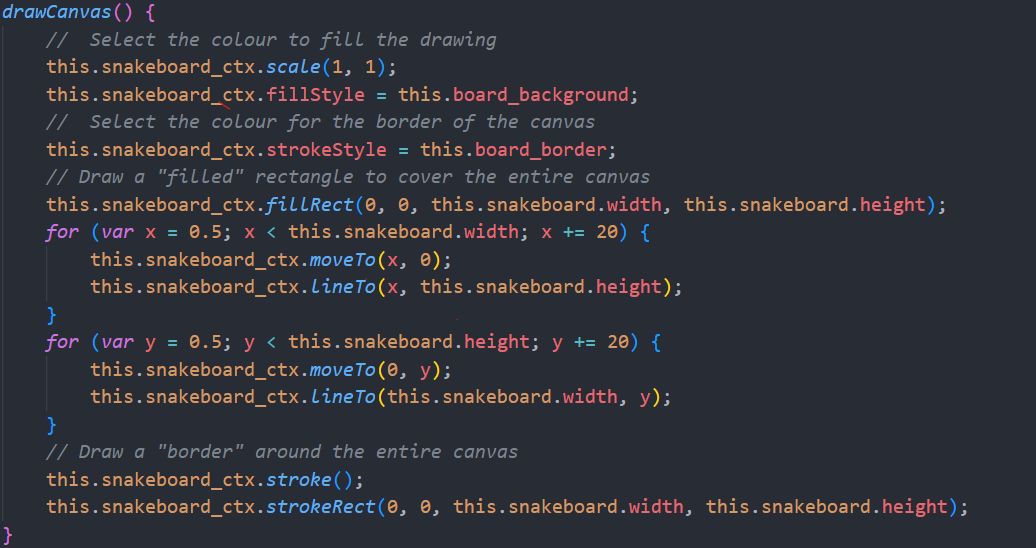
\includegraphics[scale=0.6]{chapters/hinh/snake6.png}
\end{figure}

\subsection{Xử lý va chạm}
\begin{itemize}
    \item Ta kiểm tra nếu rắn đụng đầu vào tường hay tự cắn chính mình bằng cách xem tọa độ đầu có trùng với tọa độ viền hay tọa độ thân rắn hay không. Nếu hai tọa độ trùng nhau => Trò chơi kết thúc.
\end{itemize}
\begin{figure}[ht]
    \centering
    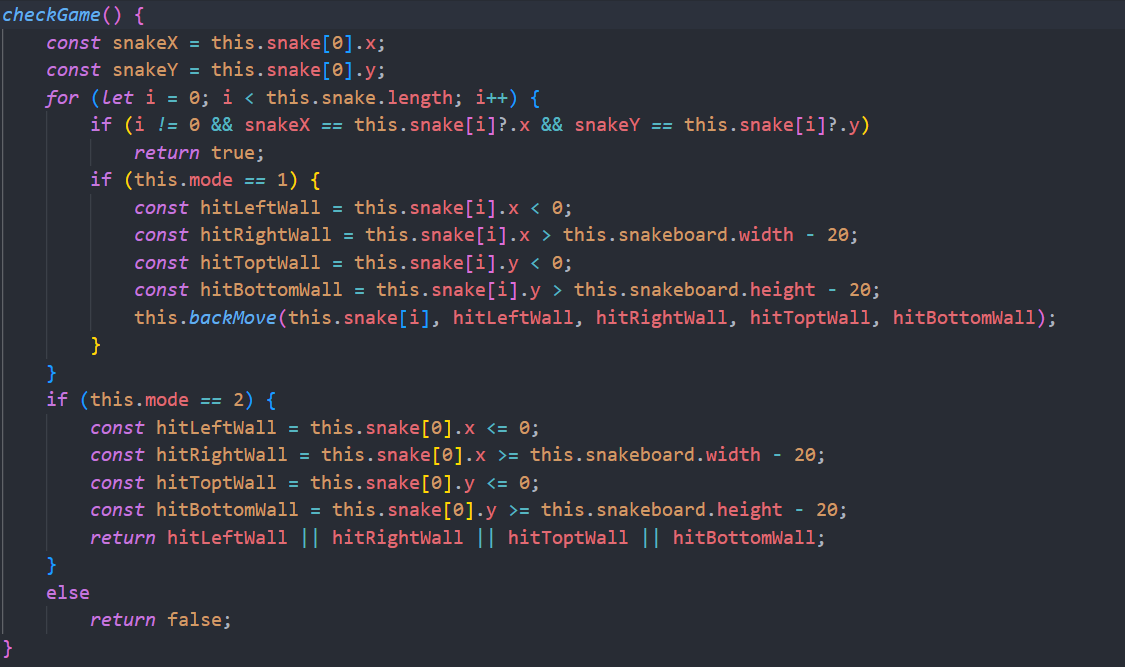
\includegraphics[scale=0.6]{chapters/hinh/snake2.png}
\end{figure}
\begin{itemize}
    \item Để kiểm tra rắn có ăn được quà hay không, ta kiểm tra tọa độ phần đầu của con
rắn và tọa độ của quà. Nếu cả hai tọa độ trùng nhau (tức là rắn ăn được mồi) thì tăng chiều dài con rắn và cộng thêm 1 điểm, quà sẽ mất và tạo ngẫu nhiên quà ở vị trí mới.
\end{itemize}
\begin{figure}[ht]
    \centering
    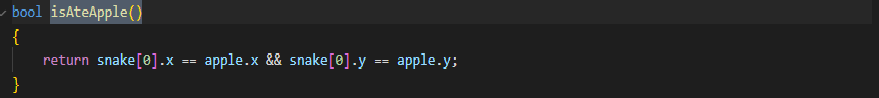
\includegraphics[scale=0.6]{chapters/hinh/snake3.png}
\end{figure}

\subsection{Tạo menu}
\begin{itemize}
    \item Menu sẽ gồm 2 lựa chọn: “Bắt đầu” (phím 1) và “Thoát” (phím 2).
    \item Nếu chọn "Bắt đầu": người chơi sẽ lựa chọn level từ 1 đến 5 (lần lượt từ phím 1 đến phím 5) và bắt đầu chơi. Người chơi có thể thoát bất cứ lúc nào bằng cách chọn phím ’q’.
    \item Nếu chọn "Thoát": trò chơi sẽ kết thúc.
\end{itemize}
\begin{figure}[ht]
    \centering
    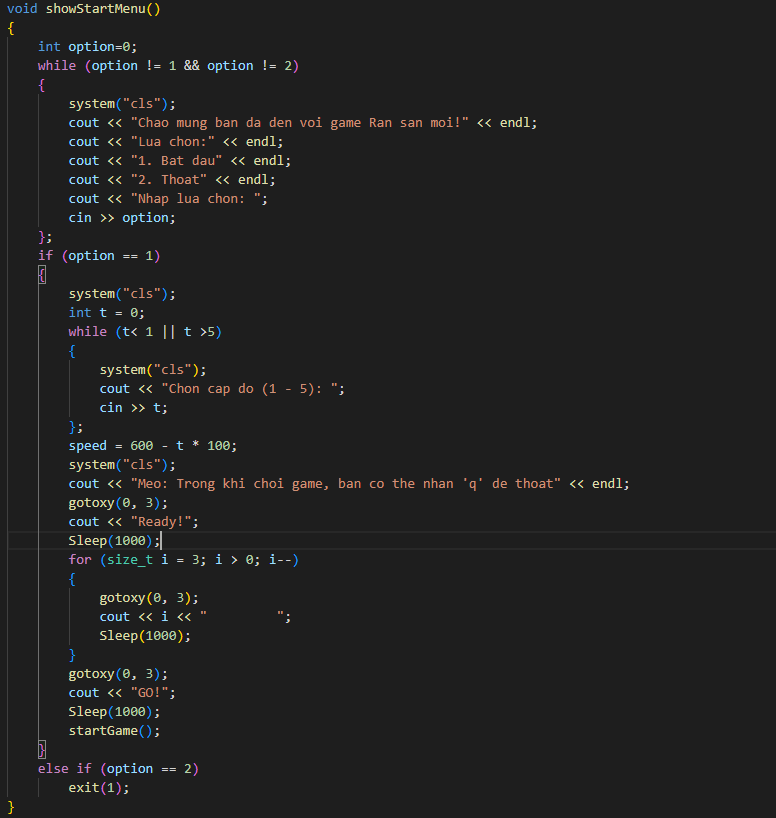
\includegraphics[scale=0.6]{chapters/hinh/snake4.png}
\end{figure}
\begin{itemize}
    \item Sau khi kết thúc màn chơi (hoàn thành màn chơi hoặc thua do rắn đụng đầu vào tường/rắn tự cắn chính mình), người chơi có thể nhấn phím ’y’ để chơi tiếp hoặc nhấn phím ’n’ để thoát trò chơi.
\end{itemize}
\begin{figure}[ht]
    \centering
    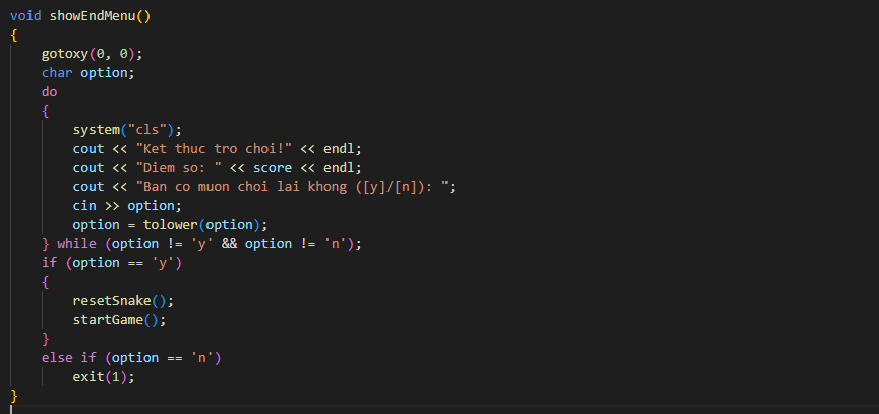
\includegraphics[scale=0.5]{chapters/hinh/snake5.png}
\end{figure}
\end{document}
